\documentclass[Bachelorarbeit.tex]{subfiles}
\begin{document}

\graphicspath{{./figures/interpretation/}}	%specifying the folder for the figures

\chapter{Interpretation}
In this chapter interpretation of the results of Chapter \ref{ch:results} "Results" are given and discussed where the central question is whether the ascending-connected topology satisfies the hypothesis or not. Thus only the Ascending-Connected topology is handled - both with and without importance sampling - because it is the most minimal network which satisfies the requirements for the hypothesis. The Hub-, Scale-Free and Small-World Topologies are handled in appendix \ref{app:interpretation} as they turn out to fall far from satisfying the hypothesis because almost all of them do not satisfy the requirements for the hypothesis. Special treatment is given to Erdos-Renyi and Watts-Strogatz as they satisfy the hypothesis when using specific parameters for their generating algorithms.

\section{Validating the Hypothesis}
When looking at the results of ascending-connected topology with and without importance sampling from Chapter \ref{ch:results} "Results" of figure \ref{fig:wealth_ASCENDINGCONNECTED_IS_100_NOCOLLATERALMARKET_REPL} and \ref{fig:wealth_ASCENDINGCONNECTED_100_NOCOLLATERALMARKET_REPL} and comparing it with the results of the fully-connected topology of figure \ref{fig:wealth_FULLYCONNECTED_100_NOCOLLATERALMARKET_REPL} it becomes immediately clear that the equilibrium is different from the equilibrium of the fully-connected network and thus theoretical equilibrium is not reached in the case of ascending-connected topology neither with or without importance sampling. Although the visual results come quite close to the fully-connected one - there is a clear distinction between pessimists, medianists and optimists and the wealth-distribution looks about the same as in fully-connected - there remain artefacts in the range of the pessimists. Thus the hypothesis is proven wrong by experiment.

\section{Analysing artefacts}
Obviously the artefacts in the range of the pessimists indicate a miss-allocation of wealth, which are in fact collateralized assets. Pessimists, as noted in Chapter \ref{ch:leverace_cycle} "The Leverage Cycle", are maximally short on assets and bonds and hold only cash, thus it is clearly a miss-allocation. As will be shown it comes from the fact that the pessimists want to sell but no neighbour is able to buy any more - a scenario which is not possible in fully-connected topology and is thus unique to ascending-connected networks with or without importance sampling.

\subsection{Dynamics of a single run}
To better understand how such artefacts arise one needs to investigate the dynamics of a single run of ascending-connected topology.

\begin{figure}[H]
	\centering
  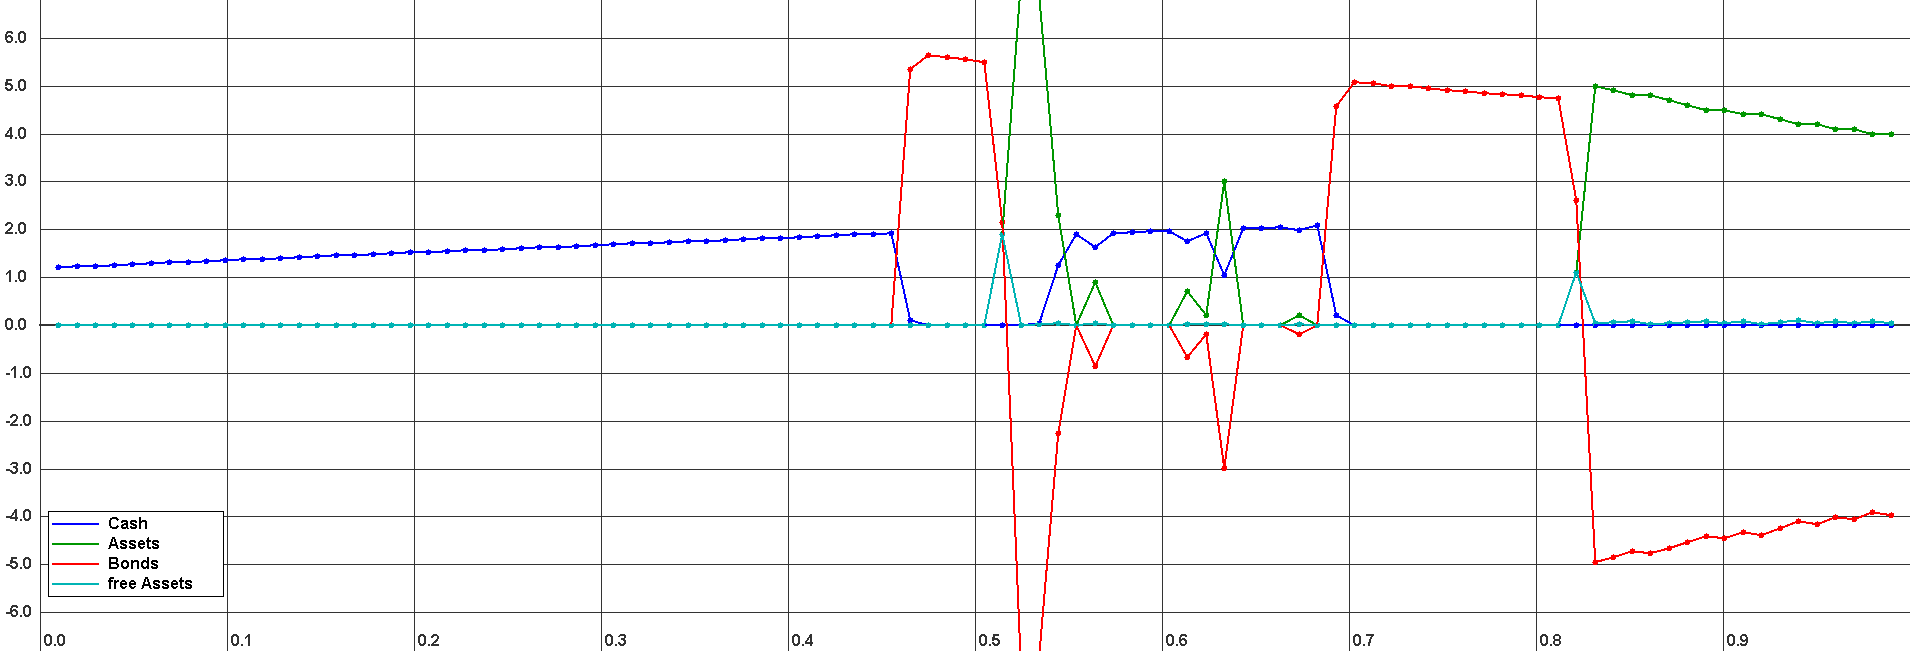
\includegraphics[width=1.0\textwidth, angle=0]{ASCENDINGCONNECTED_100_NOCOLLATERALMARKET_SINGLE.png}
	\caption{Wealth-Distribution of Ascending-Connected topology after a single run}
	\label{fig:wealth_ASCENDINGCONNECTED_IS_100_NOCOLLATERALMARKET_SINGLE}
\end{figure}

\medskip 

The wealth stabilizes from both the left and the right end of the optimism-scale towards the i1-point where medianists become optimists - around this point the last trades will happen.

\medskip 

Pessimists try to sell all their assets against cash to the neighbour with higher optimism-factor.

\medskip 

Optimists try to buy as much assets as they can get from the neighbour with lower optimism-factor. In the beginning they use cash and after they've ran out of cash they buy assets against bonds.

\medskip 

The medianists serve as connection between the pessimists and optimists, serving in transferring the assets to the optimists by buying from lower optimism and selling to higher ones either through asset against cash or asset against bond.

\medskip 

Thus the assets move from the pessimists through the ascending chain of optimism to the optimists as no direct connection between these two groups exists with the medianists in between. Thus waves of uncollateralized assets can be seen moving from pessimists to optimists.

\medskip 

It is important to understand that all agents despite their optimism factor make offers on all markets if they are able to, e.g. cash, collateral or bond constraints satisfied. This implies that pessimists trade bonds as well as assets against bonds - the agents are not defined exogenous as pessimists/medianist/optimists but this property is emerges during the simulation.

\medskip 

Thus pessimists gain wealth in collateralized assets which can be seen by the green spikes with the same amount of negative bonds as those assets are bought against bond - see Chapter \ref{ch:leverage_cycle}. Of course they try to sell it to neighbours with higher optimism factor but this is only possible if these neighbours are able to buy which they can if they hold enough bonds to buy the offered asset for the offered amount of bonds.

\medskip 

Whether an agent has enough wealth to buy from a seller is more or less random and depends on its trading history. Matching happens randomly and thus it is possible that the neighbourhood of a seller "dries up" as the potential buyers sold all their good to the next agent with higher optimism factor and become thus unable to buy from the potential seller because they have no more bonds to buy assets against bonds. In such a case a potential pessimist seller of collateralized assets is then cut from its environment and becomes unable to trade any more resulting in a miss-allocation in collateralized assets.

\medskip 

It is also possible for a group of agents to get cut from its environment through this random trading-process. In this case this "island" of agents still trades between each other resulting in the uncollateraliziing of assets which immediately are traded towards optimists but as soon as a point is reached where no buyer is available with enough bonds to buy collateralized assets this island is also incapable of trading any more resulting in an island of miss-allocated wealth.

\medskip 

An important fact to notice is that the artefacts must not necessarily show up. It is possible for a single run to finish without these artefacts showing up. This is due to the random-process of sweeping and matching and thus the artefacts are subject to this random process too. Importance sampling elevates this problem a bit as it allows for more trades as the matching probabilities are very much increased but fails in the end for the same reason as the simulation without it - the artefacts are just "smaller" but show up almost always.

\section{Extending the Hypothesis}
After it has become clear that the hypothesis is wrong the question arises what needs to be done to correct the it. It is clear that a mechanism needs to be found which prevents or resolves the arising of the artefacts within the pessimist wealth-range. Obviously two solutions are available.

\subsection{Approaching fully connectedness}
Increasing the connectedness of the topology increases the probability of global-optimal trades and allows more agents to trade between each other and thus the probability of resolving islands or artefacts of wealth miss-allocation is increased with the density of connectedness.
The experiments of ascending-connected topology with short-cuts were desigend to get an understanding how the simulation behaves with increasing connectedness and also how the two types fully and regular of connectedness influence the results.
It seems that full shortcuts seem to help dramatically although the number of full shortcuts seem to be dependent on the number of agents.
TODO: verweis auf results und interpretation appendixe

Of course in real environments approaching fully connectedness is not always possible and thus only the other mechanism is left as an option to resolve the artefacts.

\subsection{Re-Enabling trading}
Another way to look at the arising of the artefacts is because of suboptimal trades. \cite{Breuer2015} were confronted with this circumstance when they introduced the "Asset against Bond" Market where they found that the equilibrium was fundamentally different from theoretical one because agents were trapped in suboptimal trades and couldn't reverse their decisions made earlier. As a solution they introduced the "Bonds-Pledgeability" (BP) mechanism which allows to trade bonds in both ways instead of only gathering them and not being able to sell them - see \ref{ch:leverage_cycle} for a more in-depth discussion of the BP-Mechanism.

\medskip 

Thus if those artifacts are treated as suboptimal trades one needs to introduce a mechanism similar to BP to allow the reversibility of suboptimal trades in the context of collateralized assets. The only possibility without altering the network-topology is to re-enable the pessimists to trade their collateralized assets against cash as all pessimists hold cash and are thus able to buy and sell collateralized assets against cash. This new mechanism is expected to repair the miss-allocated wealth and to restore the validity of the previously disproved hypothesis.

\medskip 

See Chapter \ref{ch:new_market} "A new Market" for the implementation and results of this new mechanism.

\end{document}
